För att evaluera verktyget används existerande verktyg som jämförelse i
kombination med att dess fördelar och nackdelar vägs mot AMBA. Dessutom
presenteras en diskussion kring utvecklingsprocessens gång och
vidareutvecklingspotential.

\section{Jämförelse mellan AMBA och Ghidra} Ghidra är ett avancerat verktyg som
gör statisk analys bortom syftet med AMBA, men AMBA har ett par likheter. Ghidra
kan representera en kontrollflödesgraf för en given binär på två olika sätt:
\textit{Flow Graph} och \textit{Code Flow Graph}~\cite{ghidra_website}.

\begin{figure}[H]
    \begin{subfigure}{0.3\textwidth}
        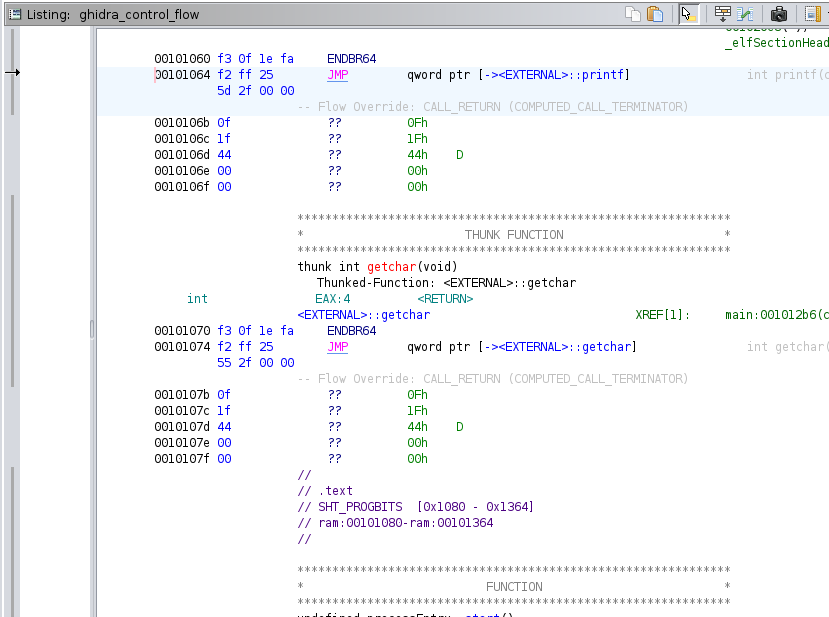
\includegraphics[width=\linewidth]{figures/ghidra_code_listing.png}
        \caption{Ghidras code listing.} \label{fig:ghidra_code_listing}
    \end{subfigure}
    \hspace*{\fill}
    \begin{subfigure}{0.3\textwidth}
        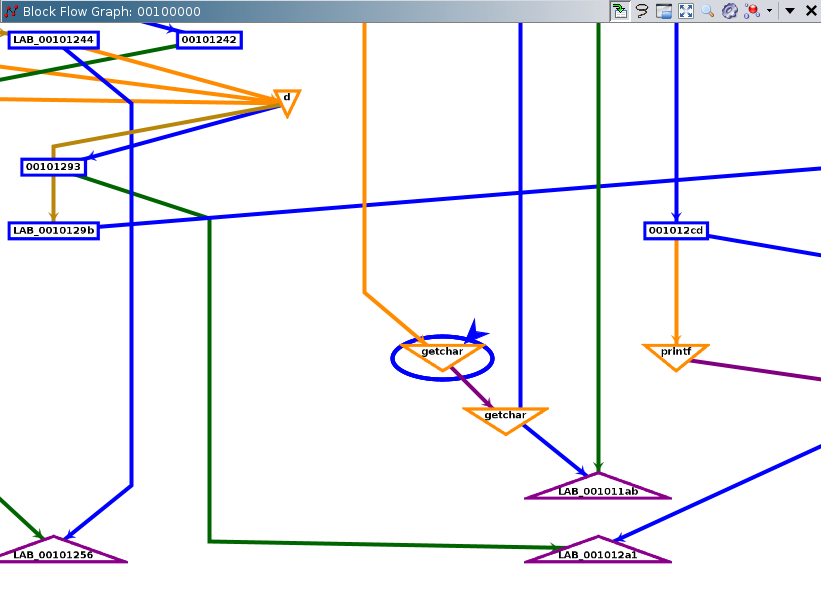
\includegraphics[width=\linewidth]{figures/ghidra_block_flow_graph.png}
        \caption{Ghidras block-flow-graph.}
        \label{fig:ghidra_block_graph}
    \end{subfigure}
    \hspace*{\fill}
    \begin{subfigure}{0.3\textwidth}
        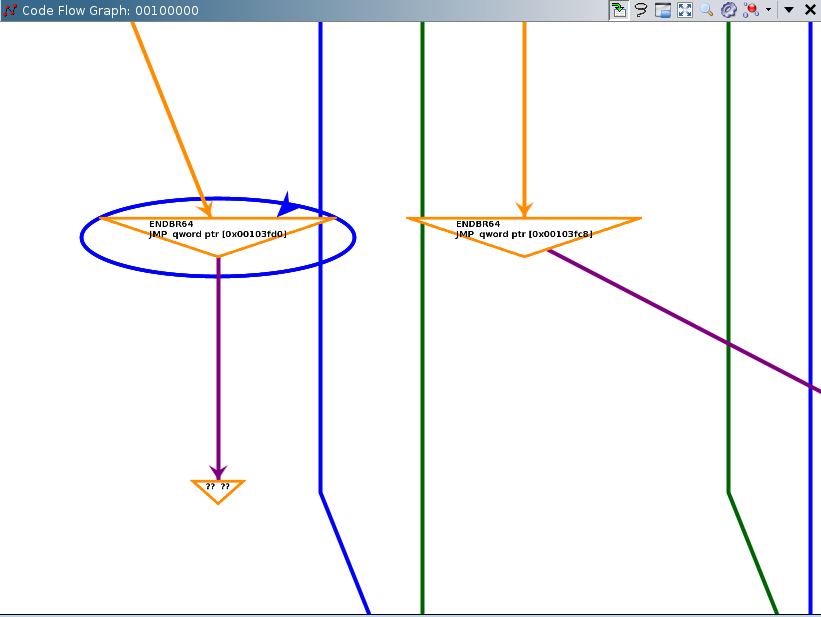
\includegraphics[width=\linewidth]{figures/ghidra_code_flow.png}
        \caption{Ghidras code-flow-graph.} \label{fig:ghidra_code_flow_graph}
    \end{subfigure}

    \caption{Tre primära vyer i verktyget Ghidra för att representera ett programs
        kontrollflödesgraf.} \label{fig:ghidra_figures}
\end{figure}

Ghidra kompletterar dessa vyer med en \textit{code listing}, en primär vy där
binärens disassemblerade kod listas. Användaren kan fritt välja att bilda en
graf från ett markerat \textit{code block}, vilket är Ghidras utökade
specifikation på ett basic block, från Ghidras code
listing~\cite{ghidra_website}. AMBA har liknande funktionalitet, se
figur~\ref{fig:graf-basic}, och kan visualisera binärens fullständiga
disassemblerade kod för en given nod, om debugdata finns tillgänglig, men saknar
större kontext likt Ghidras code listing. En fördel mot Ghidras representation
är AMBAs tre olika sätt att representera en binärs kontrollflöde på: \textit{Raw
    Basic Block Graph}, \textit{Compressed Block Graph}, och \textit{State Graph}.
Genom att använda dessa tre olika vyer kan en användare bilda en större
förståelse om en given binär, dels genom att exempelvis visualisera alla
symboliska tillstånd som \stoe{} skapar i kombination med färgade noder som
indikerar på starkt kopplade komponenter (jfr. eng. \emph{strongly connected
    components}).

Kännedom om starkt kopplade komponenter i en kontrollflödesgraf är i synnerhet
intressant vid analys av binärer utan källkod, eftersom dessa delgrafer speglar
en starkare koppling mellan noderna och indikerar på en sektion i binären som
troligtvis har större relevans än en sektion som saknar eller har betydligt
färre starkt kopplade komponenter. Ett typiskt mönster man kan se med starkt
kopplade komponenter är icke-nestlade loopar.

TODO Screenshot för node coloring som tas upp nedan TODO

En användare skulle exempelvis kunna använda AMBAs node colouring för att bilda
en större uppfattning om en viss del i binären och sedan komplettera med
nodernas minnesaddresser för att visualisera samma sektion i ett mer avancerat
verktyg som Ghidra. Ett typiskt användningsfall skulle kunna vara att i Ghidra
söka efter strängar som ger mer information i den givna kodsektionen från AMBA
eller använda Ghidras analysmetoder för att dekompilera binärens instruktioner
till ett mer läsbart format i form av pseudokod.

\section{Jämförelse mellan S2E och Angr som \\ backend} Eftersom AMBA använder
\stoe{} som symbolisk exekveringsmotor har AMBA således en teoretisk fördel i
prestanda, något som kan avläsas från figurerna
i~\cite[Figur~1-5]{systematic_comparison_symbex}. Detta innebär att AMBA inte nödvändigtvis i
nuläget har bättre prestanda mot applikationer utvecklade med Angr som
\emph{backend}. Dock betyder det att AMBA har en teoretisk konkurrenskraftig
prestanda.

Angr är dock ett mer flexibelt verktyg som har den funktionalitet som \stoe{}
tillhandahåller, och är dessutom i allmänhet enklare att påbörja utveckling med
och onekligen eklare att bygga. Dessutom är Angr i synnerhet ett eftertraktat
verktyg att använda som symbolisk exekveringsmotor eftersom det bland annat
tillhandahåller funktionalitet såsom \emph{Control-Flow Graph Recovery} och
disassemblering som möjliggör mycket av funktionalitet som annars behövs
implementeras i AMBA.

\section{Jämförelse mellan AMBA och SymNav} SymNav tillhandahåller samma
funktionalitet som AMBA gör bortsett från en detalj: användare kan genom SymNav
ta bort states som inte är intressanta medan i AMBA kan användare prioritera
states som ska analyseras. Dessutom presenteras funktionaliteten i SymNav på ett
mer användarvänligt sätt: vyn splittar upp respektive funktionalitet i
applikationen och presenterar detta i stil med designmönstret \emph{Grid of
    equals}.

Utöver detta är den stora skillnaden vilken symbolisk exekveringsmotor som
används. SymNav använder Angr, och AMBA använder, som tidigare nämnt, \stoe{}
vilket innebär att SymNav får en enklare kodbas eftersom mycket av koden som
interagerar med Angr är pythonskript likt API-anrop vilket kräver mindre total
kod för att uppnå samma sak som med \stoe{} men är istället begränsad i
skalbarhet. \stoe{} har inbyggda plugins som tillhandahåller mycket
funktionalitet, till exempel \emph{ExecutionTracer} som övervakar och
registrerar information längs med exekveringen för en given branch vilket
tillåter en att undersöka vad som orsakar path explosion eller vilken branch som
gör flest förgreningar.

\section{Arbetsprocess}
Eftersom \stoe{} är ett komplext system med många komplicerade
biblioteksberoenden ansågs det tidigt i arbetsprocessen att göra AMBA mer
tillgängligt till slutanvändaren genom att paketera alla bibliotek som krävs för
att köra \stoe{}. Detta var en komplicerad och tidskrävande uppgift eftersom
mycket av \stoe{}s byggsystem var tvunget att återimplementeras eller kringgås
när tvetydiga och icke-triviala problem uppstod. Ett sådant problem var
nedladdningen och byggningen av guest images som \stoe{} lagrades på Google
Drive där lösningen var att istället ladda ner färdiga guest images.

Denna del av arbetet ledde till att mycket av planeringen blev förskjutet och
således fanns det mindre tid till att utveckla all funktionalitet som var tänkt.

\section{Vidareutveckling} En särskilt eftertraktad funktionalitet är
\textit{State merging}. Syftet med state merging är att minska antalet
exekveringsvägar genom att förena symboliska tillstånd som är ekvivalenta. Ett
förslag är att ge uppgiften till användaren att interaktivt välja vilka
tillstånd som sammanfogas. Således ökar prestandan för den symboliska
exekveringen som gör det möjligt att skicka fler förfrågningar (jfr. eng.
\emph{queries}) till SMT-lösaren.

Övervakning av systemanrop (jfr. eng. \emph{syscalls}) ger användaren en större
insikt i vad som sker i en specifik del av grafen, exempelvis om det sker
inmatning eller utmatning, om en process signaleras att stängas av, om binären
kör ett exec-systemanrop för att köra ett externt program, etc. är anledningar
som gör det intressant att övervaka systemanrop. För att implementera detta i
AMBA bör det undersökas om det finns hooks för detta.

I nuläget sparas inte resultatet för ett givet path constraint
och därför får användaren inte heller mer informatiom om vilken input som ledde
till att vägen nåddes i exekveringen. Optimalt hade varit om användaren kunde se
vilken indata som ledde till en särskild väg för fortsatt analys. \stoe{} har
denna information, men i nuläget sparas den inte av AMBA. Dessutom hade det
varit intressant för användare om en SMT-lösare användes för att lösa ett givet
path constraint och därmed få indata som leder till att den vägen tas i
exekveringen.
